\documentclass[11pt,a4paper]{article}

\usepackage[margin=0.8in]{geometry}
\usepackage[T1]{fontenc}
\usepackage{lmodern}
\usepackage{enumitem}
\usepackage{graphicx}
\usepackage{xurl}
\usepackage[hidelinks]{hyperref}
\usepackage{microtype}

\setlength{\parindent}{0pt}
\setlength{\parskip}{5pt}
\setlist[itemize]{leftmargin=1.4em,itemsep=2pt,topsep=2pt}
\setlist[enumerate]{leftmargin=1.6em,itemsep=2pt,topsep=2pt}

\title{\textbf{Research Proposal}}
\author{Richard Harnisch}
\date{\today}

\begin{document}

\maketitle
\vspace{-1em}

\section*{Summary}

Data centers can act as a destabilizing force in electricity grids because they focus electricity load both in time and space, violating the load diversity assumption. One example of this is when six short voltage depressions in the Eastern Interconnection caused approximately 1.5~GW of data-center load to transfer away from the grid in July 2024. The North American Electric Reliability Corporation (NERC) warns that fast and large load losses losses can create frequency and voltage risks as large voltage-sensitive loads proliferate~\cite{nerc2025incident}. Low-voltage ride-through (LVRT) requirements address this problem by specifying the voltage-time region in which a facility must remain connected. Such a requirement in fact already exists for transmission-connected demand facilities in Denmark~\cite{energinet2024tr343}.

Phythesis introduces a simulation-guided design pattern in which a large language model (LLM) generates data-center designs and revises them using physics-simulation feedback~\cite{li2026phythesis}. It applies this pattern to room layout, cooling assets, and power usage effectiveness. Unfortunately, the simulation code does not seem to be publicly available. At the same time, Xie et al. develop an open simulator and voltage controllers that improve data-center LVRT, but they evaluate a fixed facility configuration~\cite{xie2026lvrt}. So we have a dynamic LLM-centered design system informed by physical simulations, and a simulator for LVRT requirements. But we have no LLM-centered design system informed by a LVRT simulator. This is the central idea of my proposal.

I propose a Phythesis-style LLM generation-and-reflection loop coupled to the LVRT simulator. The study will use one fixed data-center network topology and one ride-through specification. A candidate design will count as successful only if it is structurally valid, obeys all modeled resource limits, and remains connected in every prescribed fault simulation. Among successful designs, the objective is to minimize the total grid-interactive uninterruptible power supply (UPS) and battery energy storage system (BESS) capacity.

We can then compare the design chosen by GridPhy with designs generated by traditional methods of data center design. An improvement would constitute a lower total UPS and battery inverter requirement.

\section{Motivation and Research Gap}

The motivation for this research centers around avoiding grid-stability incidents such as the July 2024 example. A failed lightning arrester caused six normally cleared faults, each lasting 42--66 milliseconds and depressing local voltage to 0.25--0.40 per unit~\cite{nerc2025incident}. Despite not being disconnected by the operator, controllers on the consumer-side disconnected about 1.5~GW of data center load to backup power. This shows that in large institutional consumers, it is necessary to manage power consumption in a grid-stable manner on the consumer side.

Ride-through concerns whether a large load can remain connected during disturbances that develop over milliseconds to seconds. Denmark's Energinet's Technical Regulation 3.4.3 gives us a concrete requirement to serve as a reference point for our study. At the point of connection, a facility must remain connected in the specified undervoltage fault ride-through region, including recovery to 0.90 per unit by 1.5 seconds~\cite{energinet2024tr343}. This can be seen in Figure~\ref{fig:energinet}.

\begin{figure}[htbp]
    \centering
    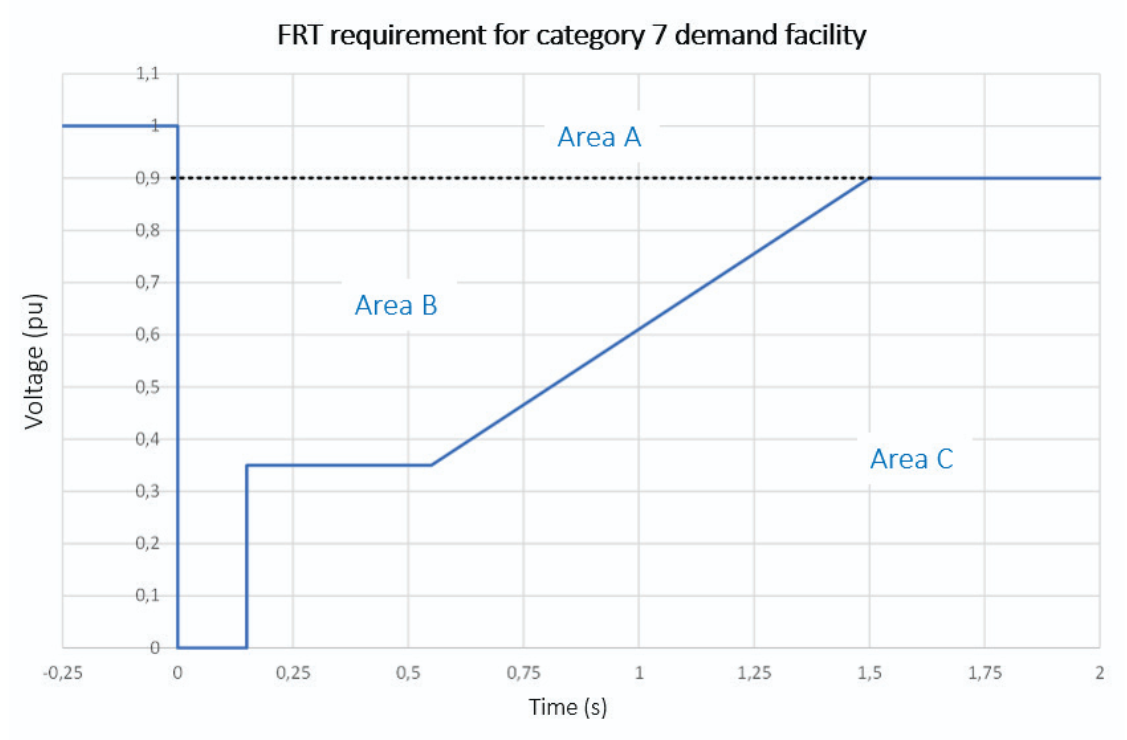
\includegraphics[width=0.8\textwidth]{energinet.png}
    \caption{Energinet's ride-through requirements. Facilities must remain connected within area B and may disconnect in area C.}
    \label{fig:energinet}
\end{figure}

Xie et al. show that active- and reactive-power control from UPS units, BESSs, computing loads, and cooling loads can prevent tripping internal protection systems which disconnect the data center from the grid. Their test system couples a radial data-center distribution network to the IEEE 14-bus transmission system and supports centralized and decentralized control~\cite{xie2026lvrt}. However, the resource locations and capacities are fixed before control is evaluated. The unanswered design problem is how much controllable capacity should be enabled, where it should be allocated, and which supported controller configuration should be used.

A note at this point: I need to spend more time understanding the Xie paper here. So far I understand the basic idea, but am not fully comfortable with it yet.

Optimizing systems using LLM agents has been researched in the past. Optimization by prompting shows that an LLM can propose new candidates from previously evaluated solutions and their objective values~\cite{yang2024opro}, while the Scientific Generative Agent framework combines LLM proposals with simulation feedback for physical discovery~\cite{ma2024sga}. Phythesis applies a similar bi-level pattern to data-center scene synthesis~\cite{li2026phythesis}. The proposed research contribution is to evaluate whether this can be transferred to data center optimization with regard to LVRT.

\section{Objective, RQ, and Hypothesis}

The primary objective is to determine whether a Phythesis-style, simulation-guided LLM loop can co-design data-center flexibility resources and controller configurations for LVRT:

\begin{quote}
    \textbf{RQ:} Given a fixed data-center electrical topology, does a Phythesis-style LLM generation-and-reflection loop find an Energinet-UV-FRT-compliant UPS/BESS allocation and controller configuration with less enabled inverter capacity than random search and conventional evolutionary search?
\end{quote}

The hypothesis is that language-based reflection on fault trajectories and prior design outcomes will guide the search toward compliant, lower-capacity configurations faster than conventional design algorithms like random sampling or evolutionary search. A negative result still would show that the added LLM does not improve the search compared to a conventional optimizer.

The study will retain the 14-bus system and the radial data-center topology from the public LVRT simulation implementation, which can be found at \url{https://github.com/caltech-netlab/datacenter-voltage-control}. The topology contains eight computing clusters with local UPS units, a central cooling plant, and two utility-scale BESS locations~\cite{xie2026lvrt}.

For each UPS and BESS location, a candidate will select whether grid-interactive control is enabled and set its available active- and reactive-power limits up to the published nameplate bounds. It will also select a controller and the supported controller parameters. For decentralized control, analytically stated stability conditions will be enforced before simulation. The primary size measure will be the sum of enabled inverter apparent-power ratings, in MVA, across the selected UPS and BESS resources.

\section{Proposed Method}

\subsection{Reproduce and parameterize the LVRT experiment}

I will first reproduce the no-control, centralized-control, and decentralized-control cases from the public implementation. The simulator supports prerecorded point-of-connection voltage traces and a coupled ANDES dynamic model~\cite{xie2026lvrt,cui2021andes}. Reproduction will establish the reference trajectories, trip behavior, available parameters, and computational budget before the search methods are introduced.

I will then expose only the UPS/BESS capacities, allocations, and supported controller choices described above. A common adapter will translate every method's candidate representation into the same simulator inputs and return the same result record: validation status, trip status, voltage trajectories, resource-limit violations, enabled capacity, and control effort.

\subsection{Define the candidate representation and validator}

Candidates will use a machine-readable schema. The schema will identify resources by fixed network location and provide bounded capacities and controller parameters. A deterministic validator will reject malformed output, nonexistent assets, capacity mismatches, out-of-range values, and controller settings that violate known stability constraints. The LLM will propose designs, but it will not decide whether they are valid or compliant. Automatic repair is excluded from the core method so that invalid-generation rates remain visible.

\subsection{Implement the simulation-guided generation loop}

The proposed loop follows the high-level organization of Phythesis and the evaluated-history principle used by OPRO~\cite{li2026phythesis,yang2024opro}:

\begin{enumerate}
    \item A design agent receives the fixed requirement, resource catalog, candidate schema, and selected previous results.
    \item The agent returns a bounded batch of structured candidate configurations.
    \item The deterministic validator accepts or rejects each candidate.
    \item The LVRT backend simulates valid candidates under the development disturbance set.
    \item Candidates are ranked by compliance first and enabled inverter capacity second.
    \item A reflection agent receives concise evidence for each failure, including the triggering bus, trip time, voltage trajectory summary, saturated resources, and controller delay. It recommends specific changes for the next iteration.
    \item The highest-ranked candidates and their feedback are supplied to the next generation until the fixed budget is exhausted.
\end{enumerate}

Prompts, model versions, sampling settings, candidate records, validation results, and simulator outputs will be logged. This makes the sequence auditable and allows failures to be attributed to generation, validation, or physical evaluation.

\section{Evaluation}

\subsection{Disturbance sets}

The development set will contain the published generator-loss case and a predefined grid of perturbations to initial data-center load, fault severity, fault duration, and centralized-controller delay, limited to ranges supported by the reproduced model. The final values will be frozen after simulator reproduction and before optimization experiments begin. A separate held-out set will use unseen combinations and boundary cases. Search feedback will never include held-out outcomes.

The Energinet UV-FRT curve will be the only regulatory envelope used for the core evaluation. Each simulated point-of-connection trace will first be classified against that curve. The no-trip obligation will be applied only where the regulation requires the demand facility to remain connected~\cite{energinet2024tr343}. This separates failure of the data-center design from a disturbance for which disconnection is permitted.

\subsection{Comparison methods}

The primary comparisons are random search and a conventional evolutionary algorithm over the same bounded representation. Both receive the same candidate and simulator budgets as GridPhy. One-shot LLM generation, which receives the requirements but no simulation history, will serve as an ablation of reflection. The published fixed-resource centralized and decentralized cases will provide domain reference points, but not search-method baselines.

The evolutionary baseline will use standard selection, crossover, and mutation without natural-language feedback. Hyperparameters for all methods will be fixed using separate pilot runs. No method may use held-out scenarios for prompt changes, hyperparameter selection, or candidate ranking.

\subsection{Analysis}

The main reported results will be the compliant-run proportion and the distribution of best compliant capacity after a fixed budget. Capacity-versus-simulator-call curves will show whether any advantage appears early or only after many evaluations. At least 20 independent runs will be used for each stochastic method. Bootstrap confidence intervals will quantify differences without relying only on a single best run.

Invalid-output rate, maximum voltage deviation, control effort, and wall-clock time will be reported to explain the primary result. They will not be used to redefine success after the experiments. An ablation without the reflection step will test whether improvement comes from iterative use of simulation evidence rather than from LLM sampling alone.

\section{Expected Contribution and Limitations}

The expected contribution is a focused empirical answer to the research question: whether a Phythesis-style LLM feedback loop adds value to constrained LVRT resource-and-controller search when compared fairly with conventional methods. The supporting artifact will consist of the candidate schema and validator, an adapter for the public LVRT simulator, the generation-and-reflection implementation, and reproducible experiment records.

The study will not establish that a generated configuration is safe to deploy. The underlying work uses a Linear DistFlow approximation for the internal data-center network and an IEEE test transmission system; controllable-device dynamics, detailed protection behavior, battery state of charge, and vendor constraints are simplified or absent~\cite{xie2026lvrt}. Consequently, the results will be evidence about search behavior within this simulator, not physical validation, regulatory certification, or a construction recommendation.

The Phythesis implementation is not publicly available as of September 2026. The project therefore reimplements only its published generation, simulation-feedback, ranking, and reflection pattern rather than claiming a direct software extension. If the LVRT code cannot reproduce the published cases, the project will stop at documenting that gap before drawing comparative conclusions. If it reproduces them but some proposed design variables cannot be parameterized reliably, those variables will be fixed rather than replaced with unverified models.

\begin{thebibliography}{9}

    \bibitem{nerc2025incident}
    North American Electric Reliability Corporation,
    \emph{Incident Review: Considering Simultaneous Voltage-Sensitive Load Reductions},
    Jan. 2025.
    \url{https://www.nerc.com/globalassets/our-work/reports/event-reports/incident_review_large_load_loss.pdf}

    \bibitem{energinet2024tr343}
    Energinet,
    \emph{Technical Regulation 3.4.3: Requirements for Transmission-Connected Demand Facilities, Revision 1},
    Sept. 2024.
    \url{https://en.energinet.dk/media/bkpf4hef/technical-regulation-343-requirements-for-transmission-connected-demand-facilities-revision-1.pdf}

    \bibitem{li2026phythesis}
    M. Li, R. Wang, R. Tan, and Y. Wen,
    ``Phythesis: Physics-Guided Evolutionary Scene Synthesis for Energy-Efficient Data Center Design via LLMs,''
    in \emph{Proceedings of the 17th ACM International Conference on Future and Sustainable Energy Systems (e-Energy)}, 2026.
    \url{https://arxiv.org/abs/2512.10611}

    \bibitem{xie2026lvrt}
    Y. Xie, W. Cui, and A. Wierman,
    ``Enhancing Data Center Low-Voltage Ride-Through,''
    in \emph{Proceedings of the 17th ACM International Conference on Future and Sustainable Energy Systems (e-Energy)}, 2026.
    \url{https://arxiv.org/abs/2510.03867}

    \bibitem{yang2024opro}
    C. Yang, X. Wang, Y. Lu, H. Liu, Q. V. Le, D. Zhou, and X. Chen,
    ``Large Language Models as Optimizers,''
    in \emph{Proceedings of the International Conference on Learning Representations (ICLR)}, 2024.
    \url{https://arxiv.org/abs/2309.03409}

    \bibitem{ma2024sga}
    P. Ma, T.-H. Wang, M. Guo, Z. Sun, J. B. Tenenbaum, D. Rus, C. Gan, and W. Matusik,
    ``LLM and Simulation as Bilevel Optimizers: A New Paradigm to Advance Physical Scientific Discovery,''
    in \emph{Proceedings of the 41st International Conference on Machine Learning},
    vol.~235, pp.~33940--33962, 2024.
    \url{https://proceedings.mlr.press/v235/ma24m.html}

    \bibitem{cui2021andes}
    H. Cui, F. Li, and K. Tomsovic,
    ``Hybrid Symbolic-Numeric Framework for Power System Modeling and Analysis,''
    \emph{IEEE Transactions on Power Systems}, vol.~36, no.~2, pp.~1373--1384, 2021.

\end{thebibliography}

\end{document}
